\section{Аналитический раздел}

\subsection{Формализация задачи}

Для организации работы магазина электроники необходимо хранить в базе данных информацию о всех товарах, представленных в каталоге, о поставщиках товаров, о клиентах, осуществлявших заказы, а также о самих заказах.

Клиент магазина должен иметь возможность просматривать каталог товаров, настраивать фильтры по интересующим его параметрам, добавлять товары в корзину, редактировать содержимое корзины и оформлять заказы. 

У сотрудника магазина должна быть предусмотрена возможность просматривать каталог товаров, историю продаж, список покупателей и список поставщиков, а также добавлять информацию о новых товарах и поставщиках. 

Чтобы начать работу в информационной системе магазина, сотрудник должен будет авторизоваться в приложении доступа к базе данных под своей учетной записью.
Поэтому для обеспечения безопасности доступа к данным магазина необходимо предусмотреть должность администратора, осуществляющего управление аккаунтами доверенных пользователей.

Таким образом, необходимо разработать программу, предоставляющую интерфейс для получения сведений магазина электроники и совершения с ними действий, доступных в зависимости от роли пользователя.

\subsection{Формализация данных}

Основная функция магазина электроники – реализация товара, поэтому товар является ключевым объектом в проектируемой базе данных. О каждом товаре необходимо хранить следующую информацию:

\begin{itemize}[leftmargin=0.7cm + \labelwidth - \labelsep]
	\item[---] наименование;
	\item[---] категория;
	\item[---] производитель;
	\item[---] страна производства;
	\item[---] поставщик;
	\item[---] цена;
	\item[---] срок гарантии;
	\item[---] количество на складе.
\end{itemize}

Также магазину удобно иметь список поставщиков товаров для дальнейшего сотрудничества. Основными данными поставщика являются:

\begin{itemize}[leftmargin=0.7cm + \labelwidth - \labelsep]
	\item[---] название организации;
	\item[---] адрес;
	\item[---] номер телефона.
\end{itemize}

Информацию обо всех осуществленных заказах было бы целесообразно сохранять для сбора статистики и ведения отчетности предприятия. Основные данные о заказе:

\begin{itemize}[leftmargin=0.7cm + \labelwidth - \labelsep]
	\item[---] товары и их количество;
	\item[---] покупатель;
	\item[---] сумма;
	\item[---] адрес доставки;
	\item[---] дата оформления.
\end{itemize}

Также имеет смысл хранить информацию о клиентах магазина, а именно:

\begin{itemize}[leftmargin=0.7cm + \labelwidth - \labelsep]
	\item[---] имя;
	\item[---] номер телефона;
	\item[---] общая сумма покупок.
\end{itemize}

Для обеспечения безопасности одновременного доступа к базе данных необходимо хранить информацию о доверенных пользователях (сотрудниках магазина), в частности:

\begin{itemize}[leftmargin=0.7cm + \labelwidth - \labelsep]
	\item[---] логин;
	\item[---] пароль;
	\item[---] имя;
	\item[---] фамилия;
	\item[---] должность;
	\item[---] адрес электронной почты.
\end{itemize}

\pagebreak

На основании описанных данных составлена ER-диаграмма, которая представлена на рисунке \ref{analysis:ershop}.

\begin{figure}[H]
	\centering{
		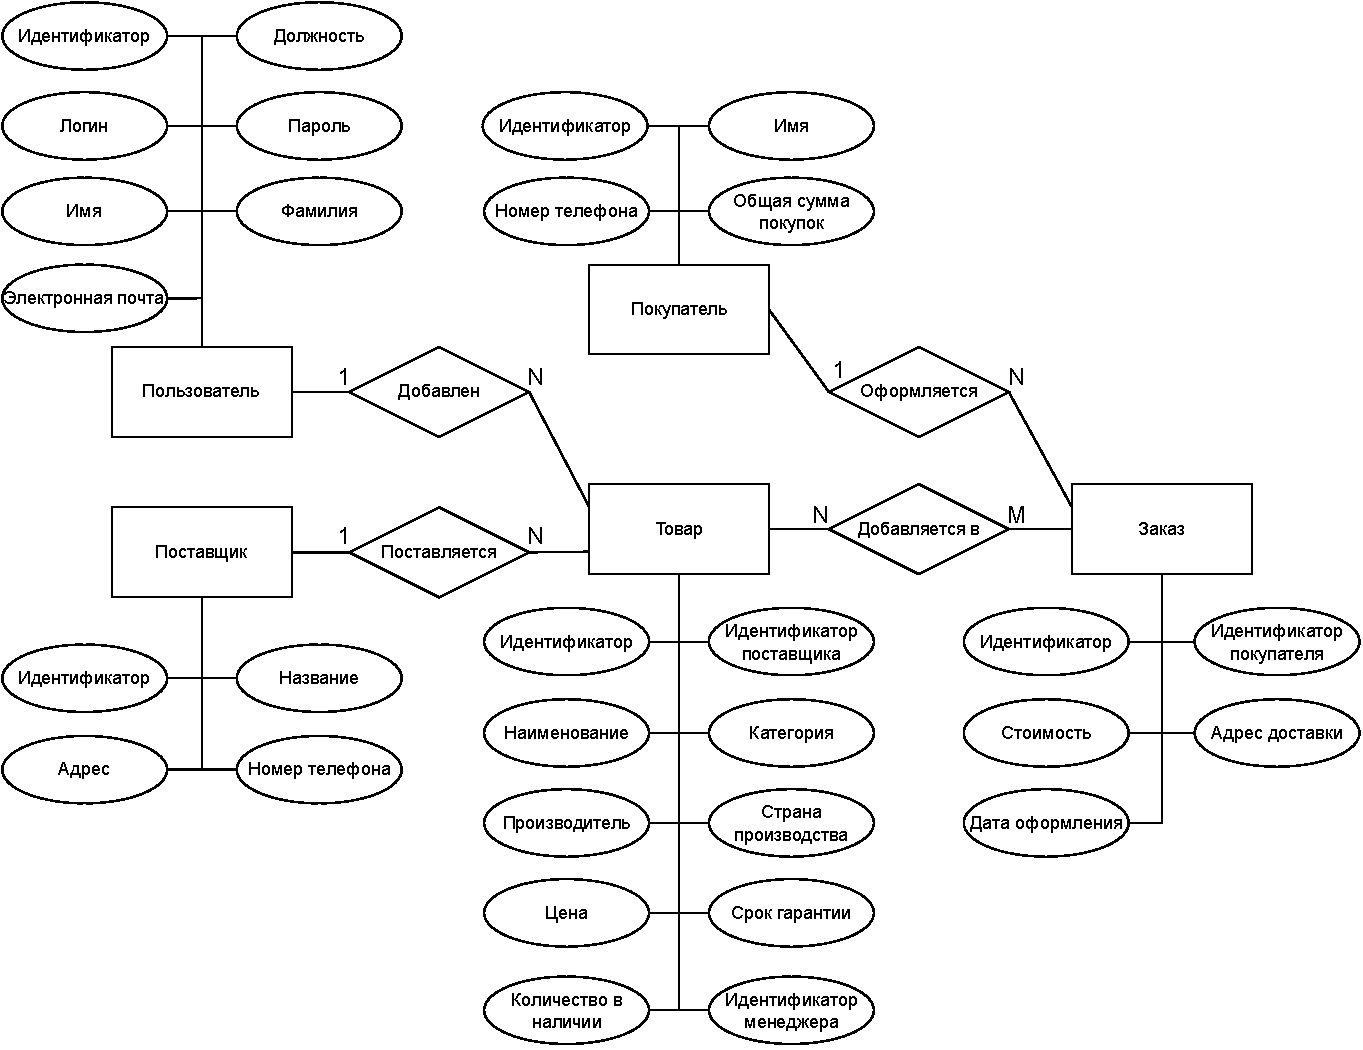
\includegraphics[width=1\textwidth]{img/erdiag.pdf}
		\caption{ER-диаграмма системы}
		\label{analysis:ershop}}
\end{figure}

\pagebreak

\subsection{Пользователи системы}

Чтобы обеспечить безопасность доступа к базе данных магазина, выделены следующие типы пользователей системы: клиент, менеджер и администратор. Для описания функционального назначения системы составлены диаграммы вариантов использования.

Клиент – это неавторизованный пользователь. Он может просматривать каталог товаров и информацию о них, фильтровать товары по интересующим его параметрам, добавлять товары в корзину, просматривать и редактировать содержимое корзины, оформлять заказы.

Диаграмма вариантов использования для клиента магазина представлена на рисункe \ref{analysis:usecaseclient}.

\begin{figure}[H]
	\centering{
		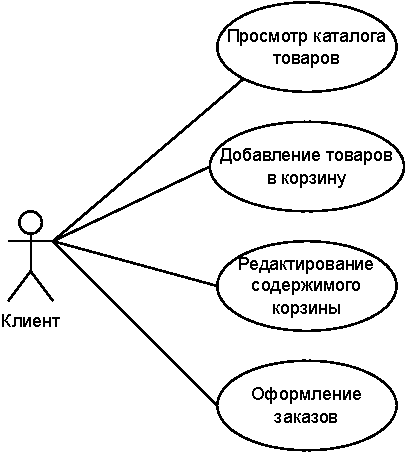
\includegraphics[width=0.65\textwidth]{img/usecaseclient.pdf}
		\caption{Диаграмма вариантов использования для клиента}
		\label{analysis:usecaseclient}}
\end{figure}

\pagebreak

Менеджер – это авторизованный пользователь. Он может просматривать каталог товаров с подробной информацией о них, историю продаж, список покупателей и список поставщиков, а также добавлять в базу информацию о новых товарах и поставщиках.

Диаграмма вариантов использования для менеджера представлена на рисункe \ref{analysis:usecasemanager}.

\begin{figure}[H]
	\centering{
		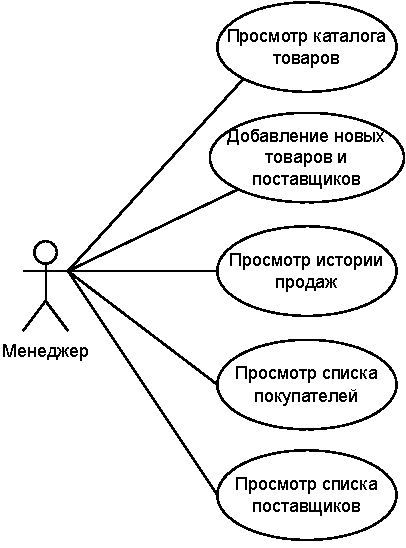
\includegraphics[width=0.65\textwidth]{img/usecasemanager.pdf}
		\caption{Диаграмма вариантов использования для менеджера}
		\label{analysis:usecasemanager}}
\end{figure}

\pagebreak

Администратор – это авторизованный пользователь. Он может просматривать список всех зарегистрированных пользователей системы, редактировать и удалять информацию о них, а также добавлять новых пользователей.

Диаграмма вариантов использования для администратора представлена на рисункe \ref{analysis:usecaseadmin}.

\begin{figure}[H]
	\centering{
		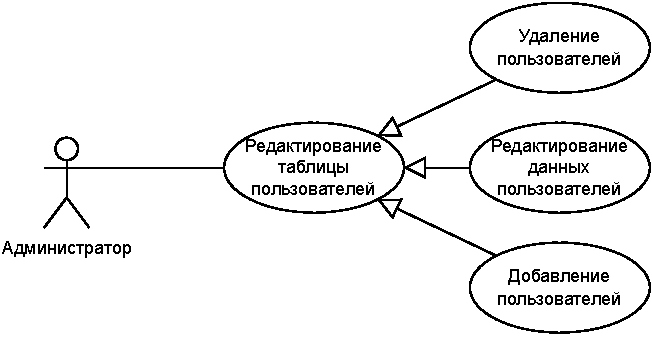
\includegraphics[width=0.9\textwidth]{img/usecaseadmin.pdf}
		\caption{Диаграмма вариантов использования для администратора}
		\label{analysis:usecaseadmin}}
\end{figure}

\pagebreak

\subsection{Анализ типов СУБД}

Система управления базами данных \cite{subd} — это набор программ, позволяющий организовывать, контролировать и администрировать базы данных.

Основными функциями СУБД являются:

\begin{itemize}[leftmargin=0.7cm + \labelwidth - \labelsep]
	\item[---] работа с внешней памятью;
	\item[---] работа с оперативной памятью;
	\item[---] журнализация изменений, резервное копирование и восстановление БД после сбоев;
	\item[---] поддержка языков БД.
\end{itemize}

\textbf{Классификация СУБД по модели данных}

Модель данных \cite{models} — это совокупность взаимосвязанных структур данных, операций над ними и множества ограничений для хранимых данных.

Основные типы моделей данных:

\begin{itemize}[leftmargin=0.7cm + \labelwidth - \labelsep]
	\item[---] иерархическая;
	\item[---] сетевая;
	\item[---] реляционная.
\end{itemize}

Иерархическая модель данных организует их в форме дерева с иерархией родительских и дочерних элементов. Такая модель подразумевает возможность существования одинаковых (чаще дочерних) элементов. При этом родительский элемент может иметь несколько потомков, но у дочернего элемента может быть только один предок.

Данные хранятся в серии записей с прикреплёнными к ним полями значений. Модель собирает вместе все экземпляры определённой записи в виде «типов записей». Для создания связей между типами записей иерархическая модель использует отношения типа «родитель-потомок» вида 1:N, что достигается путём использования древовидной структуры.

\pagebreak

Сетевая модель данных подразумевает, что у родительского элемента может быть несколько потомков, а у дочернего элемента — несколько предков. Записи в такой модели связаны списками с указателями. Сетевая модель позволяет моделировать отношения «многие ко многим», что более естественно для некоторых данных.

Основной элемент сетевой модели данных — набор, который состоит из типа «запись-владелец», имени набора и типа «запись-член». Запись подчинённого уровня («запись-член») может выполнять свою роль в нескольких наборах. Запись старшего уровня («запись-владелец») также может быть «членом» или «владельцем» в других наборах.

Главным недостатком сетевой модели данных являются жесткость и высокая сложность схемы базы данных, построенной на основе этой модели. Так как логика процедуры выбора данных зависит от физической организации этих данных, то эта модель не является полностью независимой от приложения. Иначе говоря, если будет необходимо изменить структуру данных, то нужно будет изменять и приложение.

В реляционной модели данных вся информация хранится в виде таблиц. При табличной организации отсутствует иерархия элементов. Таблицы состоят из строк – записей и столбцов – полей. На пересечении строк и столбцов находятся конкретные значения. Для каждого поля определяется множество его значений.

Данные двух таблиц связаны общими столбцами, а не физическими ссылками или указателями, в отличие от иерархической или сетевой моделей. В реляционных моделях данных нет необходимости просматривать все указатели, что облегчает выполнение запросов на выборку информации. За счет возможности просмотра строк и столбцов в любом порядке достигается гибкость выбора подмножества элементов. Реляционная модель является удобной и наиболее широко используемой формой представления данных.

\pagebreak

Для организации работы магазина необходимо обеспечить гибкость выбора случайных наборов данных. Иерархическая модель данных не отличается гибкостью и не позволяет организовать отношение «многие-ко-многим». Сетевая модель данных лишена этих недостатков, но слишком сложна и неудобна в управлении. Реляционная — более гибкая, чем иерархическая и проще для управления, чем сетевая. Учитывая перечисленные преимущества и недостатки различных моделей организации данных, была выбрана реляционная модель.

\subsection{Обзор существующих аналогов}

В открытом доступе нет приложений, которые используются сотрудниками магазинов для организации работы их предприятий. Поэтому проведем их сравнение по перечню возможностей с точки зрения клиента магазина.

Обзор возможностей приложений некоторых интернет-магазинов приведен в таблице \ref{analysis:cmpshops}.

\begin{table}[H]
	\caption{Сравнение возможностей интернет-магазинов}
	\label{analysis:cmpshops}
	\small
	\begin{tabular}{|c|cccc|}
		\hline
		\multirow{2}{*}{\begin{tabular}[c]{@{}c@{}}Название\\магазина\end{tabular}} & \multicolumn{4}{c|}{Критерий} \\ \cline{2-5} 
		& \multicolumn{1}{c|}{\begin{tabular}[c]{@{}c@{}}Поиск по\\производителю\end{tabular}} & \multicolumn{1}{c|}{\begin{tabular}[c]{@{}c@{}}Поиск по\\стране производства\end{tabular}} & \multicolumn{1}{c|}{\begin{tabular}[c]{@{}c@{}}Поиск по\\сроку гарантии\end{tabular}} & 
		\begin{tabular}[c]{@{}c@{}}Отслеживание\\количества товара\end{tabular} \\ \hline
		~123 \cite{123}~ & \multicolumn{1}{c|}{Да} & \multicolumn{1}{c|}{Нет} & \multicolumn{1}{c|}{Нет} & Да \\ \hline
		Ситилинк \cite{citilink} & \multicolumn{1}{c|}{Да} & \multicolumn{1}{c|}{Нет} & \multicolumn{1}{c|}{Частично} & Частично \\ \hline
		Лига-БТ \cite{ligabt} & \multicolumn{1}{c|}{Да} & \multicolumn{1}{c|}{Да} & \multicolumn{1}{c|}{Нет} & Нет \\ \hline
		FormulaTV \cite{formulatv} & \multicolumn{1}{c|}{Да} & \multicolumn{1}{c|}{Нет} & \multicolumn{1}{c|}{Нет} & Нет \\ \hline
	\end{tabular}
\end{table}

Как видно из приведенной таблицы, ни один из рассмотренных интернет-магазинов не удовлетворяет всем критериям.

\subsection*{Вывод}

В данном разделе были формализованы задача и данные, рассмотрены типы пользователей системы, проанализированы типы СУБД по модели данных, была выбрана реляционная модель данных. Был проведен обзор существующих решений, обозначены их недостатки.

\pagebreak